\section{Grundlagen}
\label{sec:grundlagen}

In diesem Versuch wird die Dipolrelaxation in Ionenkristallen untersucht. 
Dazu wurde ein mit Strontium-Ionen dotiertert Kalium-Bromid Kristall verwendet und seine materialspezifische Aktivierungsenergie $W$ und die charakteristische Relaxationszeit $\tau_0$ bestimmt.
\FloatBarrier

\subsection{Dipolentstehung in Ionenkristallen} % (fold)
\label{sub:dipolentstehung_in_ionenkristallen}

Ein Ionenkristall besteht aus alternierend negativ und positiv geladenen Ionen und ist nach außen somit neutral.
Wird ein solcher Kristall mit zweichfach geladenen Ionen dotiert entstehen Kationen-Leerstellen um die Ladungsneutralität aufrechtzuerhalten (Abb. \ref{fig:dipol}). 
\begin{figure}
    \centering
    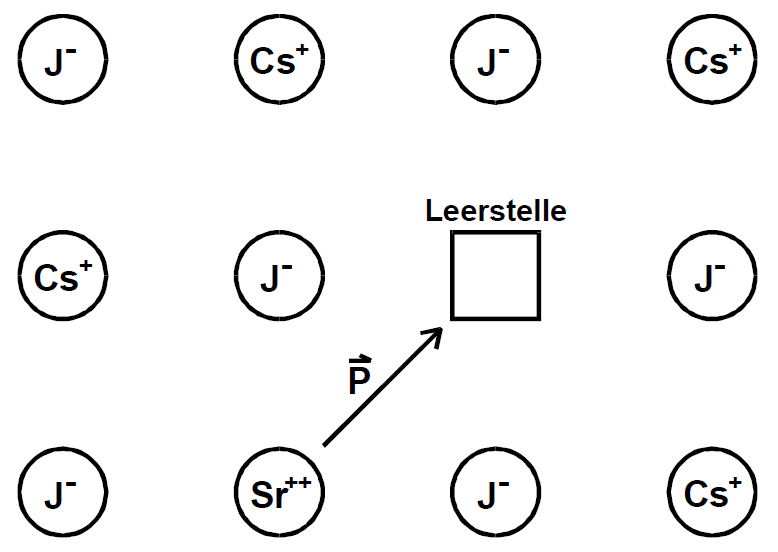
\includegraphics[width=0.5\linewidth]{img/Dipol.png}
    \caption{Entstehung eines elektrischen Dipols in einem Ionenkristall \cite{V48}.}
    \label{fig:dipol}
\end{figure}

\subsection{Richtung des Dipols} % (fold)
\label{sub:richtung_des_dipols}

Der Abstand zwischen dem zweifach geladenen Ion und der Kationen-Leerstelle gibt die Richtung des Dipols an, sodass aufgrund der Gitterplätze nur diskrete Dipolrichtungen im Kristall vorliegen können.
Unter $\SI{500}{\celsius}$ ist eine Richtungsänderung der Dipole nur durch eine Leerstellendiffusion möglich, welche uner einer materialspezifischen Aktivierungsenergie $W$ auftritt.
Der Anteil der Dipole, welche durch thermische Bewegung diese Energie aufbringen können, ist durch die Boltzmann-Statistik gegeben und somit proportional zu $\exp{\left(-W/k_\text{B}T\right)}$.
Daraus folgt für die Relaxationszeit eines Dipols der Zusammenhang
\begin{equation}
    \tau(T) = \tau_0 \exp{\left(\frac{W}{k_\text{B}T}\right)}
\end{equation}
mit der charakteristischen Relaxationszeit $\tau_0 = \tau(\infty)$.

\subsection{Messverfahren} % (fold)
\label{sub:messverfahren}

Die Probe hat eine zylindrische Form und eine Dicke von etwa $\SIrange{3}{5}{\milli\meter}$ und dient als Dielektrikum in einem Plattenkondensator.
Um die Probe zu polarisieren, wird diese über einen Zeitraum $t_{\text{pol}} \gg \tau(T)$ einem elektrischen Feld $E$ ausgesetzt.
Im Mittel wird somit ein Bruchteil $y$ der Dipole in Feldrichtung weisen, welcher näherungsweise für $pE \ll k_\text{B} T$ als
\begin{equation}
    y(T) = \frac{p E}{3 k_\text{B} T} \label{y_t}
\end{equation}
beschrieben werden kann.
Anschließend wird die Probe auf eine Temperatur $T_0$ heruntergekühlt und der Polarisationszustand somit eingefroren.
Daraufhin wird das elektrische Feld abgeschaltet und die verbleibende Ladung durch kurzschließen des Kondensators entfernt.
Wird die Probe mit konstanter Heizrate
\begin{equation}
    b := \frac{\mathrm{d}T}{\mathrm{d}t} = \text{const}
\end{equation}
erhitzt, kehren die Dipole langsam in die statistische Richtungsverteilung zurück, was als Dipolrelaxation bezeichnet wird.
Dies induziert einen Depolarisationsstrom $j(t)$, welcher in Abhängigkeit von der Temperatur zunächst steil anwächst, ein Maximum durchläuft und anschließend wieder abnimmt (Abb. \ref{fig:pol_strom}).
\begin{figure}
    \centering
    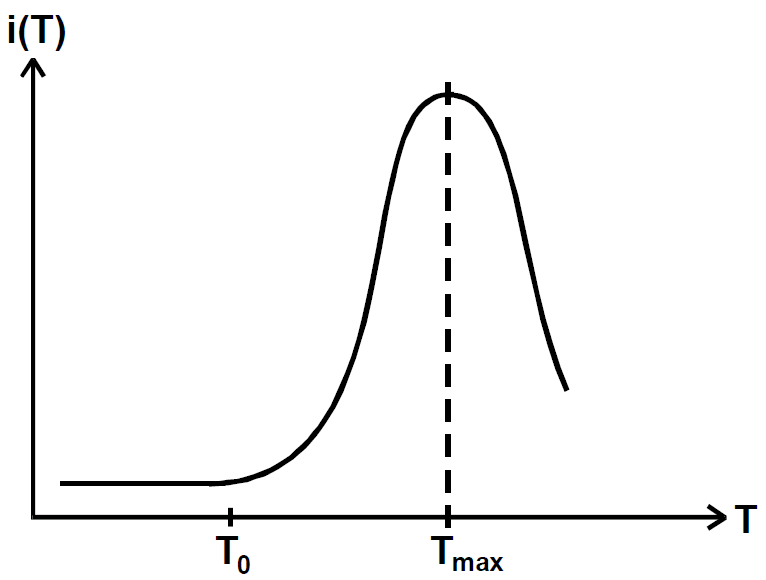
\includegraphics[width = 0.5\linewidth]{img/pol_strom.PNG}
    \caption{Der Polarisationsstrom in Abhängigkeit von der Temperatur \cite{V48}.}
    \label{fig:pol_strom}
\end{figure}
Beschrieben werden kann $j(t)$ durch
\begin{equation}
    j(t) = y(T_\mathrm{P}) p \frac{\mathrm{d}N}{\mathrm{d}t} \qquad,
\end{equation}
wobei $y(T_\mathrm{P})$ den Anteil $y$ bei der Polarisationstemperatur $T_\mathrm{P}$, $p$ das Dipolmoment und $\mathrm{d}N/\mathrm{d}t$ die pro Zeit und Volumeneinheit relaxierenden Dipole darstellt.

Mithilfe von Gleichung \eqref{y_t} ergibt sich für den Ausdruck $y(T_\mathrm{P}) p$
\begin{equation}
    y(T_\mathrm{P}) p = \frac{p^2 E}{3 k_\mathrm{B} T_\mathrm{P}} \qquad .
\end{equation}
Zudem ist die Dipolrelaxation ein thermisch aktivierter Prozess, wodurch sich für $\mathrm{d}N/\mathrm{d}t$ 
\begin{equation}
    \frac{\mathrm{d}N}{\mathrm{d}t} = -\frac{N}{\tau(T)}
\end{equation}
eine Proportionalität zu $N$ mit der Relaxationsfrequenz $1/\tau$ als Proportionalitätsfaktor einstellt.
Integration des Ausdrucks führt zu 
\begin{equation*}
    N = N_\mathrm{P} \exp{ \left( - \frac{ 1 }{ b } \int_{T_0}^T \frac{ \mathrm{d}T' }{ \tau(T') } \right )}
\end{equation*}
mit $N_\mathrm{P}$ als Zahl der zu Beginn des Aufheizens vorhandenen orientierten Dipole pro Volumeneinheit
und somit ergibt sich für den Depolarisationsstrom $j(T)$
\begin{equation}
    j(T) = \frac{ p^2 E }{ 3 k_\mathrm{B} T_\mathrm{P} } \frac{ N_\mathrm{P} }{ \tau_0 } \exp{ \left( - \frac{ 1 }{ b \tau_0 } \int_{T_0}^T \exp{ \left( - \frac{ W }{ k_\mathrm{B} T' } \right) \mathrm{d}T' } \right) } \exp{ \left( -\frac{ W }{ k_\mathrm{B} T } \right) } \label{j_t}
\end{equation}

\subsection{Berechnung der Aktivierungsenergie $W$} % (fold)
\label{sub:berechnung_der_aktivierungsenergie_w_}

Es werden zwei verschiedene Ansätze zur Berechnung der Aktivierungsenergie $W$ berechnet.

Im ersten Verfahren ist das Integral in Gleichung \eqref{j_t} etwa
\begin{equation*}
    \int_{T_0}^T \exp{ \left( - \frac{ W }{ k_\mathrm{B} T } \right )} \approx 0 \qquad , 
\end{equation*}
woraus sich der Strom näherungsweise als
\begin{equation}
    \label{eqn:approx}
    j(T) \approx \frac{ p^2 E }{ 3 k_\mathrm{B} T_\mathrm{P} } \frac{ N_\mathrm{P} }{ \tau_0 } \exp{ \left( - \frac{ W }{ k_\mathrm{B} T} \right ) }
\end{equation}
schreiben lässt.
Über eine Halblogarithmische Darstellung kann nun $W$ berechnet werden.

Im zweiten Verfahren wird $W$ über den gesamten Kurvernverlauf bestimmt.
Dazu wird genutzt, dass für die zeitliche Änderung der Polarisation
\begin{equation*}
    \frac{\mathrm{d}P}{\mathrm{d}t} = - \frac{ P(t) }{ \tau(T(t))}
\end{equation*}
gilt und diese einen äußeren Strom pro Probenquerschnitt $F$ erzeugt
\begin{equation*}
    \frac{\mathrm{d}P}{\mathrm{d}t} = \frac{j(t)}{F} \qquad.
\end{equation*}

Da $T$ eine lineare Funktion in $t$ sein soll ergibt sich aus den vorangegangenen Gleichungen
\begin{equation*}
    \tau(T) = \frac{ \int_{T}^\infty j(T') \mathrm{d}T' }{ b j(T) } 
\end{equation*}
und durch ersetzen von $\tau(T)$ 
\begin{equation}
     \frac{ W }{ k_\mathrm{B} T } = \ln{ \left( \frac{ \int_{T}^\infty j(T') \mathrm{d}T' }{ b j(T) \tau_0 } \right) } \qquad ,
\end{equation}
woraus sich nun $W$ berechnen lässt.
In der Praxis wird die obere Integrationsgrenze von $\infty$ in $T^*$ geändert, wobei $j(T^*) \approx 0$ gilt.
